\documentclass[10pt]{standalone}
\usepackage{amsmath}
\usepackage{pgf,tikz}
\usepackage{mathrsfs}
\usetikzlibrary{arrows}
\pagestyle{empty}
\begin{document}
	
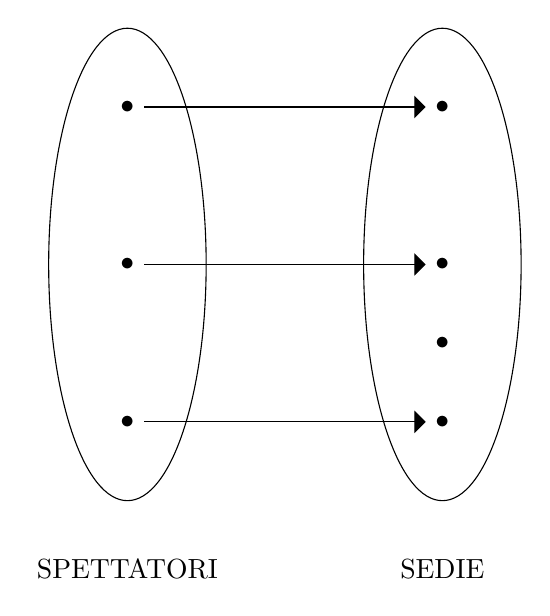
\begin{tikzpicture}
\tikzstyle{freccia} = [-triangle 90]
\draw  (0,0) node (v4) {$\bullet$} ellipse (1 and 3);
\draw  (4,0) node (v3) {$\bullet$} ellipse (1 and 3);
\node(v1) at (0,2) {$\bullet$};
\node (v5) at (0,-2) {$\bullet$};
\node (v2) at (4,2) {$\bullet$};
\node (v6) at (4,-2) {$\bullet$};
\node at (4,-1) {$\bullet$};
\draw[freccia] (v1) -- (v2);
\draw [freccia](v4) -- (v3);
\draw [freccia](v5) -- (v6);
\node[label=below:SPETTATORI] at (0,-3.5) {};
\node[label=below:SEDIE] at (4,-3.5) {};
\end{tikzpicture}
\end{document}